
\section{Cross-Branch Change Detection}
\label{main.diff-across-commits}

The change detection phase of our synchronization protocol is defined through the calls `getCommitIDsSince()' and `getChangedDataSince()'.
We will now look into the internals of the algorithms invoked through these calls.\\

\subsection{Commit History Difference}
Identifying added commit IDs since a last known synchronized commit is only working on the meta-data level - there is no application data involved in this phase.\\
Given two branches A and B we want to retrieve all commits A needs in order to be in sync with B.
Our algorithm is based on the recursive invocation of a lowest common ancestor implementation:\\

\begin{lstlisting}[caption=Detecting commit history difference, label=commit-difference]

commitA = branchA.commit
commitB = branchB.commit

\end{lstlisting}

\begin{figure}[new-commits]
  \centering
  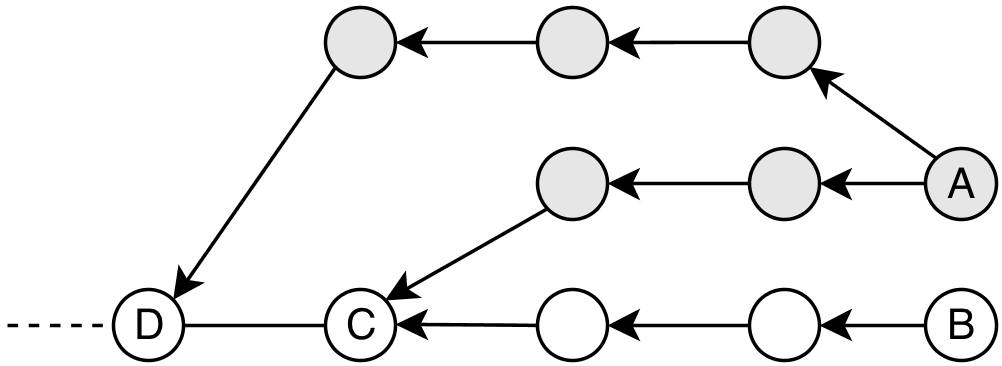
\includegraphics[width=0.6\textwidth]{img/new-commits}
  \caption{Commit difference B-A - gray commits are missing on branch B.}
  \label{fig:histo.new-commits}
\end{figure}

\subsection{Application Data Change Detection}

just use commits and identify added blobs for each by parallel tree walking of commit and ancestor...